\documentclass[String-lecture-21.tex]{subfiles}

\begin{document}
\section{T-duality}\label{sec:Tdual}


We have seen that the critical dimensions $D$ of bosonic and supersymmetric string theory are $D=26$ and $D=10$, respectively. To obtain an effective theory in lower dimensions, we can make use of \textbf{Kaluza-Klein compactifications} where  the
true spacetime takes the form of a direct product $M_{d} \times K_{D-d}$, where
$M_d$ is the $d$-dimensional Minkowski spacetime, and $K_{D-d}$ is a very tiny compact manifold. As we will see, an effective theory in $M_d$ still sees interesting ``stringy'' effects in this Kaluza-Klein scheme.




First, we concentrate on the simple compactifications, $K=T^{D-d}$
called \textrm{toroidal compactifications}.  Since a torus is simply a  product of $S^1$ and it is flat,  the nonlinear sigma model can be described by the free two-dimensional CFT. Remarkably, this simple compactification leads to the notion of \textbf{T-duality} and \textbf{Heterotic string theories} have been constructed based on toroidal compactifications as we will see in \S\ref{sec:Heterotic}. To understand the basic properties,  let us first see the toroidal compactifications of bosonic string theory. Toroidal compactifications of superstring theories are also very interesting so that we will learn about them relating to string dualities later more in detail.


The concept of D-branes was introduced as boundary conditions of open strings. T-duality gets particularly rich when we include D-branes so that we will study their properties more in detail.
The explanation of T-duality in Polchinski's lecture notes \cite{Polchinski:1996na} is so elegant that we just simply follow it in this section.


\subsection{\texorpdfstring{$S^1$}{S1} compactification in closed bosonic string}

To begin with, let us first study the simplest case of the spacetime $\bR^{1,24}\times S^1$ where we compactify 25-th direction on a circle $S^1$ of radius $R$.  For closed strings, we have the
familiar mode expansion \eqref{mode-exp}.
Now let us take a close look at the zero modes which can be written as
\[
X^{\mu}(z, \bar{z})=x^{\mu}+\bar{x}^{\mu}-i \sqrt{\frac{\alpha^{\prime}}{2}}\left(\alpha_{0}^{\mu}+\bar{\alpha}_{0}^{\mu}\right) t+\sqrt{\frac{\alpha^{\prime}}{2}}\left(\bar{\alpha}_{0}^{\mu}-\alpha_{0}^{\mu}\right) \sigma+\text { oscillators. }
\]
where the spacetime momentum of the string is
\be\nonumber
p^\mu =
\frac1{\sqrt{2\a'}}(\alpha^\mu_0 + {\ol\alpha}^\mu_0)~.
\ee

Under $\sigma \to \sigma+2\pi$,
the oscillator term is periodic and $X^\mu(z,\bar{z})$
changes by $2\pi\sqrt{(\a'/2)}(\ol\alpha^\mu_0-{\alpha}^\mu_0).$
For a non-compact spatial direction $\bR^{1,24}$, $X^\mu$ is single-valued $X^\mu(t,\s)= X^\mu(t,\s+2\pi)$,
which requires
\be\nonumber
\alpha^\mu_0={\ol\alpha}^\mu_0=\sqrt{\frac{\a'}{2}}p^\mu~,\qquad \mu=0,1,\ldots,24~.
\ee

\begin{figure}[ht]\centering
\includegraphics{picture/winding}
\end{figure}


On the other hand, since the 25-th direction is put on the circle $S^1$ of radius $R$, it has a period
 $X^{25}\sim X^{25}+2\pi R$. Hence, the momentum $p^{25}$ can take the values $n/R$ for $n\in\bZ$ where $n$ is called \textbf{Kaluza-Klein momentum}.
Also, under $\sigma\sim\sigma+2\pi$, $X^{25}(z,\bar{z})$
can change by $2\pi wR$ where $w$  is called
 the \textbf{winding number}.  Thus, we have
\[
\alpha_{0}^{25}+\bar{\alpha}_{0}^{25}=\frac{2 n}{R} \sqrt{\frac{\alpha^{\prime}}{2}}, \qquad \bar{\alpha}_{0}^{25}-\alpha_{0}^{25}=\sqrt{\frac{2}{\alpha^{\prime}}} w R
\]
implying
\begin{align}\label{25a}
\alpha^{25}_0 = \left(\frac{n}{R}-\frac{wR}{\a'}\right)
\sqrt{\frac{\a'}{2}} ~, \qquad
{\ol\alpha}^{25}_0 =
\left(\frac{n}{R}+\frac{wR}{\a'}\right)\sqrt{\frac{\a'}{2}}~.
\end{align}

Now let us study their mass spectrum. The mass formula for the string with one dimension compactified on a circle can be interpreted from a 25-dimensional viewpoint in which one regards each of the Kaluza-Klein momenta, which are given by $n$, as distinct particles. Thus, the mass formula is given by
\[M^2 = -\sum_{\mu=0}^{24}p^\mu p_\mu \]
where $\mu$ runs only over the non-compact dimensions.
Hence, we can write the mass formula as
\[
M^{2}=\frac{n^{2}}{R^{2}}+\frac{w^{2} R^{2}}{\alpha^{\prime 2}}+\frac{2}{\alpha^{\prime}}(N+\bar{N}-2)~.
\]
where $N$ and $\ol N$ are the right and left number operators \eqref{numbering}. Using \eqref{25a}, we can express the difference between the two expressions
\be\label{level-matching}
N-\ol N=nw~,
\ee
so that the level matching condition is modified due to the $S^1$ compactification. In a similar fashion, the mass can be expressed in terms of the Kaluza-Klein momentum and the winding number
\be\label{mass}
M^2=\frac{n^2}{R^2}+\frac{w^2R^2}{\a'^2}+\frac2{\a'}(N+\ol N-2)
\ee




The mass spectra \eqref{mass} of the theories at radius $R$ and $\a'/ R$ are identical
when the winding and Kaluza-Klein modes are interchanged
$n \leftrightarrow w$. This symmetry of the bosonic string theory is called \textbf{T-duality}.
From the viewpoint of strings, a circle of radius $R$ is equivalent to that of radius $\a'/ R$, and this is the main reason why we can avoid UV divergence in string theory. This shows that strings see geometry in an unprecedented and intriguing way, and this is one of the remarkable phenomena called ``stringy geometry''.




It is easy to see from \eqref{25a} that this interchange amounts to
\be
\alpha_{0}^{25} \rightarrow-\alpha_{0}^{25}, \quad \bar{\alpha}_{0}^{25} \rightarrow \bar{\alpha}_{0}^{25}
\label{tzemo}.
\ee
In fact, it is not just the zero mode, but the entire right-moving part of the compact coordinate that flips the sign under the T-duality transformation
\be
X^{\prime25}(z,\bar{z})=-X^{25}(z)+\overline X^{25}(\bar{z})\ . \label{onesidep}
\ee
Remarkably, the energy-momentum tensor, OPEs and therefore all of the correlation
functions are invariant under this rewriting. In other words, T-duality, relating the two theories with radius $R$ and $\a'/R$, is an exact
symmetry of perturbative closed string theory.

Because of the T-duality, a theory with compactification radius $R$ is equivalent to the theory with compactification radius $\a'/R$. Thus, this implies that there is a ``minimal radius'' $R=\sqrt{\a'}$ in string theory which is called \textbf{self-dual radius}. At self-dual radius, the duality
$R \to \a'/R$ maps $R$ back to its original value where we can expect
something interesting to occur.  In the next section, we will study physics at the self-dual radius.





\subsubsection*{Self-dual radius: $R = \protect \sqrt {\a'}$}

As we know, the massless spectra of bosonic string theory include gravitons. Hence, let us see the effect of the $S^1$ compactification on the gravitons. In the Kaluza-Klein mechanism  $M_{25}\times S^1$, the metric is decomposed into compact and non-compact spacetime direction
\be\label{KK-metric}
ds^2 = G_{MN} dx^M dx^N = G_{\mu\nu} dx^\mu dx^\nu + G_{25,25}(dx^{25}+ A_\mu dx^\mu)^2 ~.
\ee
where the fields $G_{\mu\nu}$, $G_{25,25}$, and $A_\mu$ are allowed to depend only on the non-compact coordinates $x^\mu$ ($\mu=0,1,\ldots24$). Under a coordinate transformation
\[x'^{25} = x^{25} + \lambda (x^\mu)  \]
the part $G_{\mu,25}=G_{25,\mu}$ of the metric transforms as
\[A'_\mu = A_\mu - \partial_\mu \lambda~ . \]
Thus, it behaves as $\U(1)$ gauge field, and gauge transformations arise as part of the higher-dimensional coordinate transformation. On the other hand, the part $G_{25,25}$ of the metric behaves as a scalar field. Indeed, writing $G_{25,25}=e^\s$, the Ricci scalar for the metric  \eqref{KK-metric} can be written as
\[
R_{26} = R_{25} - 2e^{-\s}\nabla^2 e^\s - \frac14e^{2\s}F_{\m\n}F^{\m\n}~ .
\]
Actually, it is straightforward to see the corresponding vertex operators at generic radius $R$:
\begin{align}
\partial X^\mu \bar \partial X^\nu e^{i k\cdot X}	&\quad \longleftrightarrow \quad G_{\mu\nu}, B_{\mu\nu}, \phi \cr
\partial X^\mu \bar{\partial} X^{25} e^{i k\cdot X}, \ \partial X^{25} \bar{\partial} X^\mu e^{i k\cdot X}& \quad \longleftrightarrow \quad A^\mu\,,B_{\mu,25}\cr
\partial X^{25} \bar{\partial} X^{25} e^{i k\cdot X}&\quad \longleftrightarrow \quad  \sigma
\end{align}
where $\nu = 0, \ldots, 24$  runs the coordinate indices for $M_{25}$.  In fact, the middle line indicates that the theory has $\U(1)_\ell \times \U(1)_r$ gauge symmetry at generic radius $R$.

However, at the self-dual radius $R=\sqrt{\a'}$, the mass formula \eqref{mass} becomes
\[
M^2=\frac{1}{\a'}(n^2+w^2+2(N+\ol N-2))~,
\]
so that the massless spectra actually get enlarged. In addition to the generic solution $n=w=0$, $N=\ol N =1$, there are now
also
\begin{table}[ht]\centering
\begin{tabular}{ccccc}
&$n$&$w$&$\ol  N$&$N$\\\hline
A&$\pm1$&$\pm1$&$0$&$1$\\
B&$\pm1$&$\mp1$&$1$&$0$\\
C&$\pm2$&$0$&$0$&$0$\\
D&$0$&$\pm2$&$0$&$0$
\end{tabular}\end{table}

\noindent Hence, the states corresponding to A and B contain four new gauge bosons with vertex operators
\[
\bar{\partial} X^\mu e^{\pm 2iX^{25}(z)/\sqrt{\a'}} e^{i k\cdot X} ~,  \qquad\qquad  {\partial} X^\mu e^{\pm 2i\overline X^{25}(\bar z)/\sqrt{\a'}} e^{i k\cdot X}~.
\]
Indeed, C and D also give rise to new gauge bosons (exercise).
It is expected that the new gauge bosons must combine with the
old into a non-Abelian theory. In fact, if one can define the current
\[
j^\pm(z)=j^1(z)\pm i \, j^2(z):=e^{\pm 2iX^{25}(z)/\sqrt{\a'}} \qquad j^3(z):=i\, \partial X^{25}(z)/\sqrt{\a'}~,
\]
they satisfy the OPEs (Exercise)
\[
j^a(z) j^b (0) \sim \frac { k\delta^{ab} } {2z^2}
		+ \frac {i {\epsilon^{abc}} j^c(0)} {z}~.
\]
with $k=1$. Here $\epsilon^{abc}$ is the structure constant
of $\SU(2)$.  This is precisely the definition of $\SU(2)$ affine Lie
algebra with level $k=1$.  The same story is repeated for the left movers.  Hence we see that we have
an enhancement of gauge symmetry from $\U(1)_\ell \times \U(1)_r$
to $\SU(2)_\ell \times \SU(2)_r$ at $R = \sqrt{\a'}$.


In fact, when the theory moves away from the self-dual radius $R=\sqrt{\a'}$, the $\SU(2)_\ell \times \SU(2)_r$  gauge symmetry is Higgsed.
The world-sheet action is deformed by turning on the marginal operator
\[
V_{a\ol a}:=j_a \bar j_{\ol a} e^{ik\cdot X}~,
\]
which is equivalent to giving the VEV of the $(3,3)$-component of the Higgs field. As a result, when the theory is away from the self-dual
radius, the $\SU(2)_\ell \times \SU(2)_r$ gauge symmetry is spontaneously broken down to a $\U(1)_\ell \times \U(1)_r$.



\subsection{T-duality of open strings}\label{sec:Tdual-open}


Now let us consider T-duality on the open string spectrum in the $S^1$ compactification. At the end of \S\ref{sec:quantization}, we briefly study open string spectra. There, we learned that Neumann boundary condition on the $X^\mu$-direction is achieved by imposing $ \alpha_n^\mu = \overline{\alpha}_n^\mu$ while Dirichlet boundary condition is by $\alpha^\mu_n = -\overline{\alpha}_n^\mu$. Since T-duality along the 25-th direction transforms the modes as in \eqref{tzemo}, it therefore exchanges Neumann to Dirichlet condition \cite{Dai:1989ua,Leigh:1989jq}:
\[
\left.\partial_{\sigma} X^{25}\right|_{\sigma=0, \pi}=\left.0 \quad \rightarrow \quad \partial_{t} X^{\prime 25}\right|_{\sigma=0, \pi}=0~.
\]
Suppose that an open string with Neumann boundary condition has KK momentum $n$ along the 25-th direction, and we perform T-duality on that circle. Then, a simple calculation
\begin{align}
X^{\prime 25}(\pi)-X^{\prime 25}(0) &=\int_{0}^{\pi} d \sigma \partial_{\sigma} X^{\prime 25}=i \int_{0}^{\pi} d \sigma \partial_{t} X^{25} \\
&=2 \pi \alpha^{\prime} p^{25}=\frac{2 \pi \alpha^{\prime} n}{R}=2 \pi n R^{\prime}
. \label{deltax}
\end{align}
tells us that the $X^{25}$ coordinate of the open string endpoints is fixed after T-duality. T-duality transforms the KK momentum $n$ to winding number $n$  as in the figure below.
This can be interpreted as follows. Open strings can freely move on a space-filling D25-brane. After T-duality, the space-filling D25-brane becomes a D24-brane with its $X^{25}$ coordinate fixed. As a result, all the endpoints of open strings are constrained to the fixed $X^{25}$-direction whereas they are free to move in the other 24 spatial dimensions.
More generally, the boundary condition of open strings can be imposed at any dimension. Since T-duality interchanges Neumann and Dirichlet boundary conditions, T-duality tangent to a D$p$-brane brings it to a D$(p-1)$-brane. On the other hand, T-duality orthogonal to a D$p$-brane turns it into a D$(p+1)$-brane.




\begin{figure}[ht]\centering
\includegraphics[width=13cm]{picture/open-T-duality}
\end{figure}

We can ask a question which position of the $X^{25}$ coordinate a D24-brane is located in the figure above. This question is related to Chan-Paton factors we encountered in \S\ref{sec:intro-Dbrane}. Suppose that there are $K$ space-filling D25-branes, which give rise to $\U(K)$ spacetime gauge fields. In the current setting,
$X^{25}$ direction is compactified on the circle $S^1$ so that we can include a Wilson loop on $S^1$ as
\be
A_{25}=\textrm{diag}\{\theta_1,\theta_2,\ldots,\theta_K\}/2\pi R
\ee
The insertion of the Wilson loop breaks the gauge group as $\U(K) \to \U(1)^K$, and the broken gauge group is abelian so that we can write it as
\be\nonumber
A_{25}=-i \Lambda^{-1} \partial_{25} \Lambda, \quad \Lambda=\operatorname{diag}\{e^{i X^{25} \theta_{1} / 2 \pi R}, e^{i X^{25} \theta_{2} / 2 \pi R}, \ldots, e^{i X^{25} \theta_{N} / 2 \pi R}\}\ .
\ee
Then, under the translation $X^{25}\to X^{25}+2\pi R$, an open string state $|N=1;n;ij \rangle$ is shifted by a phase
\be
e^{i(\theta_j-\theta_i)}~,
\ee
which means its momentum is shifted by $(\theta_j-\theta_i)/2\pi$ from an integer $n$. Under T-duality, the momentum is transformed into the winding number. Therefore, $\theta_i$ can be understood as the $X^{25}$ coordinate of the $i$-th D24-brane after T-duality.
Namely, the open string state $|N=1;n;ij \rangle$ is mapped to an open string of length
\be\nonumber
X^{\prime 25}(\pi)-X^{\prime 25}(0)=\left(2 \pi n+\theta_{j}-\theta_{i}\right) R^{\prime}~.
\ee
There are in general $K$ D24-branes at different positions as schematically depicted in the following figure.
\begin{figure}[ht]\centering
\includegraphics[width=7cm]{picture/open-Higgs}
\end{figure}

Then, the $(D-1)=24$-dimensional mass of this open string is
\begin{align}
M^{2} &=\left(p^{25}\right)^{2}+\frac{1}{\alpha^{\prime}}(N-1) \\
&=\left(\frac{\left[2 \pi n+\left(\theta_{j}-\theta_{i}\right)\right] R^{\prime}}{\pi \alpha^{\prime}}\right)^{2}+\frac{1}{\alpha^{\prime}}(N-1)~ .\nonumber
\end{align}
Hence, massless gauge bosons arise only from open strings $|N=1;n=0;ii \rangle$ whose endpoints are on the same D-brane.
Due to the string tension, open strings that stretch between different D-branes become massive (gauge field). Therefore, this can be understood as the Higgs mechanism in which $X^{25}$ expectation values (coordinates) of $K$ D24-branes take different values, and the gauge group is broken as $\U(K) \to \U(1)^K$. This situation is called \textbf{Coulomb phase}, where the Goldstone bosons are ``eaten'' by gauge fields $|N=1;n=0;ij \rangle$ which become massive.


Let us make an important remark. So far, we have treated D-branes just as rigid boundary conditions. However,  D-branes are dynamical so that they can fluctuate in shape and position. As we will see in \S\ref{sec:D-brane}, \S\ref{sec:BH}, \S\ref{sec:AdSCFT}, the gravitational and gauge dynamics on a stack of D-branes makes string theory very intriguing.




\subsection{T-duality of Type II superstrings}
Let us briefly discuss how the
T-duality
 acts on Type II superstring compactified on $M_{9} \times S^1$. We have seen that the T-duality acts as the parity transformation on the right-moving sector
 \[
  {X}^9 ( z)\quad\longleftrightarrow\quad -  {{X}'^9}( z)
 \]
The superconformal invariance requires
\[\psi^9 \leftrightarrow - {\psi}^{'9}~.\]
 However, this implies that the chirality of the right-moving R sector ground state is reversed: the raising and lowering operators ${\psi}^{8}\pm i{\psi}^{'9}$ are interchanged. (See \eqref{raising-lowering}.) In other words, T-duality is a spacetime parity operation on just one side of the world-sheet, so it reverses the relative chiralities of the right- and left-moving ground states. As a result, Type IIA theory with compactification radius $R$ is T-dualized to Type IIB theory with radius $\a'/R$.

 Chiral spinors are now defined by using \eqref{Gamma11}
 \[
 \Gamma_{11} \psi_{\pm}=\pm \psi_{\pm}
 \]
and we define $\bar{\psi}_{\pm}=\psi_{\pm}^{\dagger} \Gamma^{0}$. Then, the vertex operators of the R-R field strengths $G_{\mu_{1} \cdots \mu_{p+2}}$ are expressed as spinor bilinears
  \[
  \mathrm{IIA}: \bar{\psi}_{-}^{L} \Gamma^{\mu_{1} \cdots \mu_{p+2}} \psi_{+}^{R}, \quad \mathrm{IIB}: \bar{\psi}_{+}^{L} \Gamma^{\mu_{1} \cdots \mu_{p+2}} \psi_{+}^{R}
  \]
  where $\psi^{R}\left(\psi^{L}\right)$ comes from the right (left) movers and
  \[
  \Gamma^{\mu_{1} \cdots \mu_{p+2}}=\Gamma^{[\mu_{1}} \cdots \Gamma^{\mu_{p+2}]}
  \]
  is the antisymmetric product of $(p+2)$ gamma matrices.

Since the IIA and IIB theories have different R-R fields, T-duality in the 9th direction will transform one into the other. This can be seen from the action of T-duality on the spin fields as
\be\nonumber
\psi^R_{\alpha} (z) \to  \beta_9 \psi^R_{\alpha} (z),\qquad
\overline\psi^L_{\alpha} (\bar{z}) \to\overline\psi^L_{\alpha} (\bar{z})
\ee
for $\beta_9 =\Gamma^9\Gamma^{11}$, the parity transformation (9-reflection) on the
spinors.
Hence, the R-R fields are transformed as
\begin{align}\label{RR-Tduality}
C_9 &\quad \to\quad C \cr
C_{\mu},C_{\mu \nu 9}&\quad \to\quad C_{\mu 9}, C_{\mu\nu}\cr
C_{\mu \nu \lambda}&\quad \to\quad C_{\mu \nu \lambda 9}~.
\end{align}
Figure \ref{fig:D1-D2-T-dual} illustrates the behavior of D-branes under the T-duality, and Table \ref{tab:Tdual} shows different D-brane configurations in Type II theories that are dual to each other.



\begin{figure}[ht]\centering
  \includegraphics[width=12cm]{picture/D1-D2-T-dual}
  \caption{D$1$-brane and its T-dual D$2$-brane on $\bR \times S^1$.}
  \label{fig:D1-D2-T-dual}
\end{figure}



\begin{table}[ht]\centering
  IIB \qquad
\begin{tabular}{c|cccccccccc}
& {0} & {1} & {2} & {3} & {4} & {5} & {6} & {7} & {8} & {9} \\
\hline  NS5  & $\times$ & $\times$ & $\times$ & $\times$ & $\times$ & $\times$ & & & & \\
\hline D1 & $\times$ & $\times$ &  & & & & & & &  \\
\hline D5 & $\times$ & $\times$ &  & & & & $\times$ & $\times$ & $\times$ &$\times$
\end{tabular}\\
\tikzset{every picture/.style={line width=0.75pt}}

%set default line width to 0.75pt

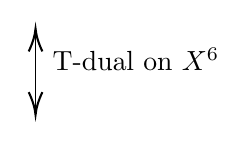
\begin{tikzpicture}[x=0.75pt,y=0.75pt,yscale=-1,xscale=1]
%uncomment if require: \path (0,300); %set diagram left start at 0, and has height of 300

%Straight Lines [id:da5202601090739447]
\draw    (203,138) -- (203,175.5) ;
\draw [shift={(203,177.5)}, rotate = 270] [color={rgb, 255:red, 0; green, 0; blue, 0 }  ][line width=0.75]    (10.93,-3.29) .. controls (6.95,-1.4) and (3.31,-0.3) .. (0,0) .. controls (3.31,0.3) and (6.95,1.4) .. (10.93,3.29)   ;
\draw [shift={(203,136)}, rotate = 90] [color={rgb, 255:red, 0; green, 0; blue, 0 }  ][line width=0.75]    (10.93,-3.29) .. controls (6.95,-1.4) and (3.31,-0.3) .. (0,0) .. controls (3.31,0.3) and (6.95,1.4) .. (10.93,3.29)   ;

% Text Node
\draw (210,144) node [anchor=north west][inner sep=0.75pt]  [align=left] {T-dual on $X^{6}$};


\end{tikzpicture}\\
 IIA \qquad
\begin{tabular}{c|cccccccccc}
& {0} & {1} & {2} & {3} & {4} & {5} & {6} & {7} & {8} & {9} \\
\hline  NS5  & $\times$ & $\times$ & $\times$ & $\times$ & $\times$ & $\times$ & & & & \\
\hline D2 & $\times$ & $\times$ &  & & & &$\times$ & & &  \\
\hline D4 & $\times$ & $\times$ &  & & & & & $\times$ & $\times$ &$\times$
\end{tabular}\\
\tikzset{every picture/.style={line width=0.75pt}} %set default line width to 0.75pt

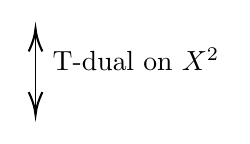
\begin{tikzpicture}[x=0.75pt,y=0.75pt,yscale=-1,xscale=1]
%uncomment if require: \path (0,300); %set diagram left start at 0, and has height of 300

%Straight Lines [id:da5202601090739447]
\draw    (203,138) -- (203,175.5) ;
\draw [shift={(203,177.5)}, rotate = 270] [color={rgb, 255:red, 0; green, 0; blue, 0 }  ][line width=0.75]    (10.93,-3.29) .. controls (6.95,-1.4) and (3.31,-0.3) .. (0,0) .. controls (3.31,0.3) and (6.95,1.4) .. (10.93,3.29)   ;
\draw [shift={(203,136)}, rotate = 90] [color={rgb, 255:red, 0; green, 0; blue, 0 }  ][line width=0.75]    (10.93,-3.29) .. controls (6.95,-1.4) and (3.31,-0.3) .. (0,0) .. controls (3.31,0.3) and (6.95,1.4) .. (10.93,3.29)   ;

% Text Node
\draw (210,144) node [anchor=north west][inner sep=0.75pt]  [align=left] {T-dual on $X^{2}$};


\end{tikzpicture}\\
  IIB \qquad
\begin{tabular}{c|cccccccccc}
& {0} & {1} & {2} & {3} & {4} & {5} & {6} & {7} & {8} & {9} \\
\hline  NS5  & $\times$ & $\times$ & $\times$ & $\times$ & $\times$ & $\times$ & & & & \\
\hline D3 & $\times$ & $\times$ & $\times$ & & & &$\times$ & & & \\
\hline D5 & $\times$ & $\times$ & $\times$ & & & & & $\times$ & $\times$ &$\times$
\end{tabular}\\
\tikzset{every picture/.style={line width=0.75pt}}  %set default line width to 0.75pt

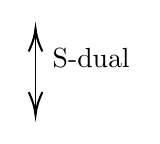
\begin{tikzpicture}[x=0.75pt,y=0.75pt,yscale=-1,xscale=1]
%uncomment if require: \path (0,300); %set diagram left start at 0, and has height of 300

%Straight Lines [id:da5202601090739447]
\draw    (203,138) -- (203,175.5) ;
\draw [shift={(203,177.5)}, rotate = 270] [color={rgb, 255:red, 0; green, 0; blue, 0 }  ][line width=0.75]    (10.93,-3.29) .. controls (6.95,-1.4) and (3.31,-0.3) .. (0,0) .. controls (3.31,0.3) and (6.95,1.4) .. (10.93,3.29)   ;
\draw [shift={(203,136)}, rotate = 90] [color={rgb, 255:red, 0; green, 0; blue, 0 }  ][line width=0.75]    (10.93,-3.29) .. controls (6.95,-1.4) and (3.31,-0.3) .. (0,0) .. controls (3.31,0.3) and (6.95,1.4) .. (10.93,3.29)   ;

% Text Node
\draw (210,144) node [anchor=north west][inner sep=0.75pt]  [align=left] {S-dual};


\end{tikzpicture}\\
 IIB \qquad
\begin{tabular}{c|cccccccccc}
& {0} & {1} & {2} & {3} & {4} & {5} & {6} & {7} & {8} & {9} \\
\hline  D5  & $\times$ & $\times$ & $\times$ & $\times$ & $\times$ & $\times$ & & & & \\
\hline D3 & $\times$ & $\times$ &  $\times$ & & & &$\times$ & & &  \\
\hline NS5 & $\times$ & $\times$ &  & & & &  & $\times$ & $\times$ &$\times$
\end{tabular}
\caption{D-branes and dualities in Type II theories. The last two configurations will appear in \S\ref{sec:HW}.}
\label{tab:Tdual}
\end{table}
\end{document}
